\documentclass[11pt]{article}
\usepackage[margin=0.85in, top=0.75in, bottom=0.6in]{geometry}
\usepackage{graphicx}
\usepackage{enumitem}
\usepackage{xcolor}
\usepackage{hyperref}
\usepackage{tgtermes}
\usepackage[T1]{fontenc}
\usepackage[numbers,sort&compress]{natbib}
\renewcommand{\bibsection}{\section*{References}}
\setlength{\bibsep}{2pt}

% Compact lists
\setlist[itemize]{nosep, leftmargin=1.5em, topsep=0.2em}
\setlist[enumerate]{nosep, leftmargin=1.5em, topsep=0.2em}

% Reduce space around section headings
\usepackage{titlesec}
\titlespacing*{\section}{0pt}{0.8em}{0.4em}

\pagestyle{empty}

\title{Agentic Scientific Instruments:\\From Distributed Cognition to Cross-Domain Discovery}
\author{P.S. Kesavan\\\texttt{pskeshu@gmail.com}}
\date{}

\begin{document}
\maketitle

\begin{abstract}
The emergence of large language models with reasoning capabilities has opened the door to agentic science---systems that perceive, reason, and act within the scientific discovery process.
While applications are appearing across fields, promising to accelerate research, surface connections inaccessible to humans, and close the loop between hypothesis and experiment, adoption has been slow.
The core difficulty is not the models themselves but fitting the right agentic patterns to the domain: the specific scientific discipline, the meta-domain of science as a practice, and the scales at which agency operates---from individual researcher to laboratory to meso-institutional.
When instruments are involved, the problem deepens into one of distributed cognition, where the culture and epistemology of science must be considered alongside the engineering.

We report on an ongoing effort to implement agentic patterns in developmental biology microscopy, where agents control sensitive instruments under safety constraints, reason multimodally over images of biological entities that span scales of space, time, and developmental state, and bridge epistemic structures not directly accessible through observation alone.
From this foundation we ask the natural next question: can agents coordinating across instruments---a hive mind with varied resources---test hypotheses grander than any single instrument could address?
Can different scientific modalities, such as microscopy and genomics, coordinate across the biological stack despite operating at fundamentally different levels?
And if epistemic patterns of nature are universal, can agents communicating across scientific domains---biology, astronomy, materials science, engineering---discover global regularities and catalyze the mixing of scientific cultures that interdisciplinary science has long promised?
We argue that realizing this vision requires infrastructure designed from the start for cross-domain agency, and that anything less is mainstream.
\end{abstract}

\section{Why Instrumentation}

Agentic patterns can be applied at many levels of science: assisting a researcher with literature, managing a laboratory workflow, or coordinating multi-site collaborations.
But instrumentation occupies a unique position.
An instrument is where theory meets matter---where hypotheses become measurements and measurements become evidence.
When an agent controls an instrument, it inherits both the power and the constraints of physical observation: safety is paramount, decisions are irreversible, and the entity under study is not a static dataset but a living, changing system.

In developmental biology microscopy, these constraints are acute.
The biological specimen exists across scales of space (subcellular to organismal), time (seconds to days), and state (a continuously developing embryo).
The agent must perceive through images, reason about what it sees in the context of what it knows, and decide what to observe next---all while operating a sensitive light-sheet microscope safely.
This is not prompt engineering; it is distributed cognition between a reasoning system and a physical instrument.

We have built \textsc{Gently}, an agentic microscope that implements this pattern (Figure~\ref{fig:domains}).
Four capability domains are operational: visual perception through vision-language model reasoning traces, adaptive multi-embryo event-driven acquisition, a multi-layer safety stack for hardware control, and lineage-tracked data provenance.
Four domains are emerging: scientific reasoning through structured campaign--hypothesis--observation hierarchies, experiment design with gap assessment, persistent memory across sessions, and distributed collaboration with peer agents.

The power of this approach lies in epistemic bridging.
The agent reasons on top of visible empirical information, connecting structures that are not accessible through microscopy alone or not observable at any given moment due to technical limitations.
It bridges what can be seen with what is known, across scales that no single observation can span.

\begin{figure}[ht]
  \centering
  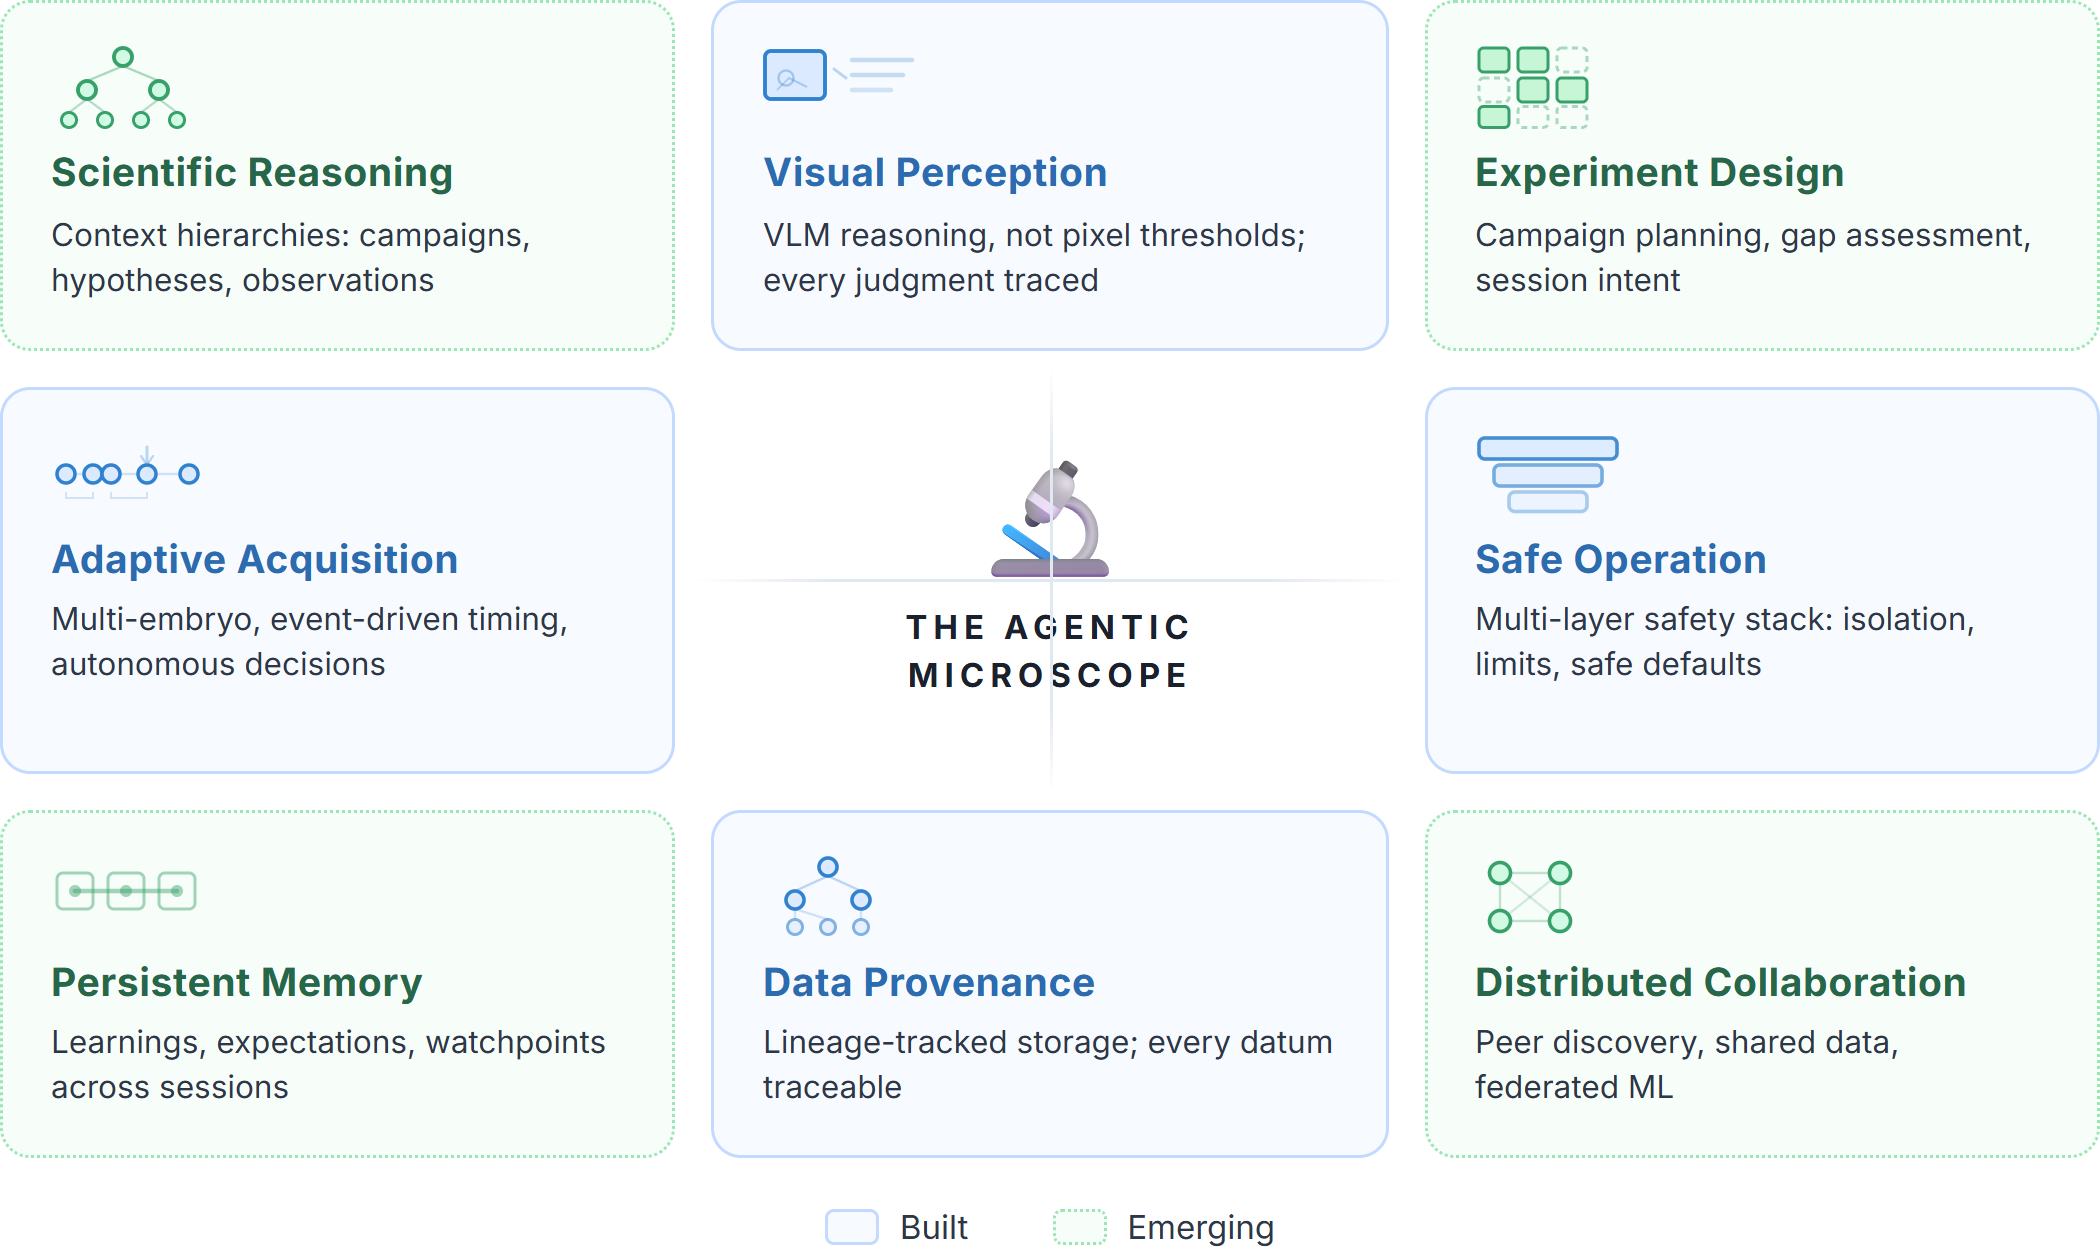
\includegraphics[width=0.75\textwidth]{diagrams/figure1_agent_domains.png}
  \caption{\textbf{Domains of the Agentic Microscope.}
  Eight capability domains of a single instrument agent.
  Blue (solid border): built and operational.
  Green (dotted border): emerging.}
  \label{fig:domains}
\end{figure}

\section{From One Instrument to a Hive Mind}

Once a single agent controls one microscope, the natural question is whether agents can cooperate across instruments.
A light-sheet microscope and a confocal microscope observe the same biology with different trade-offs.
A cryo-EM reveals ultrastructure invisible to light.
A genomics pipeline probes the same biological system at the level of genome and proteome, while microscopy operates at the phenomenological level.
These are technically different modalities, but they work on the same biological stack.
An agent that can reason across them is not merely automating parallel experiments---it is coordinating a study the way a large collaboration does, but with the speed and consistency of a computational system.

This is the vision of a hive mind: agents with varied resources---instruments, compute, trained models, accumulated knowledge---that can discover each other, understand each other's capabilities, and coordinate to test hypotheses grander than any single instrument could address.

Realizing this requires infrastructure (Figure~\ref{fig:infrastructure}, top).
We identify three layers.
\textbf{Discover}: agents find peers through decentralized peer-to-peer broadcast, with no central registry.
Every agent announces its presence; any agent can search for capabilities it needs.
\textbf{Describe}: each agent advertises what it \emph{has} (instruments, robots, compute infrastructure), what it \emph{can} do (segmentation, tracking, spectral analysis), and what it \emph{knows} (domain expertise, trained models, annotated datasets).
Other agents query this capability space to find collaborators.
\textbf{Coordinate}: agents design experiments that incorporate peer capabilities, delegating subtasks and synthesizing results into shared understanding.

With this infrastructure, what emerges is population structure (Figure~\ref{fig:infrastructure}, bottom).
Within a scientific domain, agents form dense local communities---sharing data, validating findings, training models together through federated learning.
This is \emph{local order}: the same-language collaboration that happens naturally within a field.
Across domains, sparser bridges form.
A morphological pattern detected by a microscopy agent connects to a structural motif found in materials characterization.
An adaptive observation strategy developed for telescope surveys transfers to environmental sensor networks.
This is \emph{global order}: cross-domain connections that surface regularities no single community could discover alone.

\begin{figure}[ht]
  \centering
  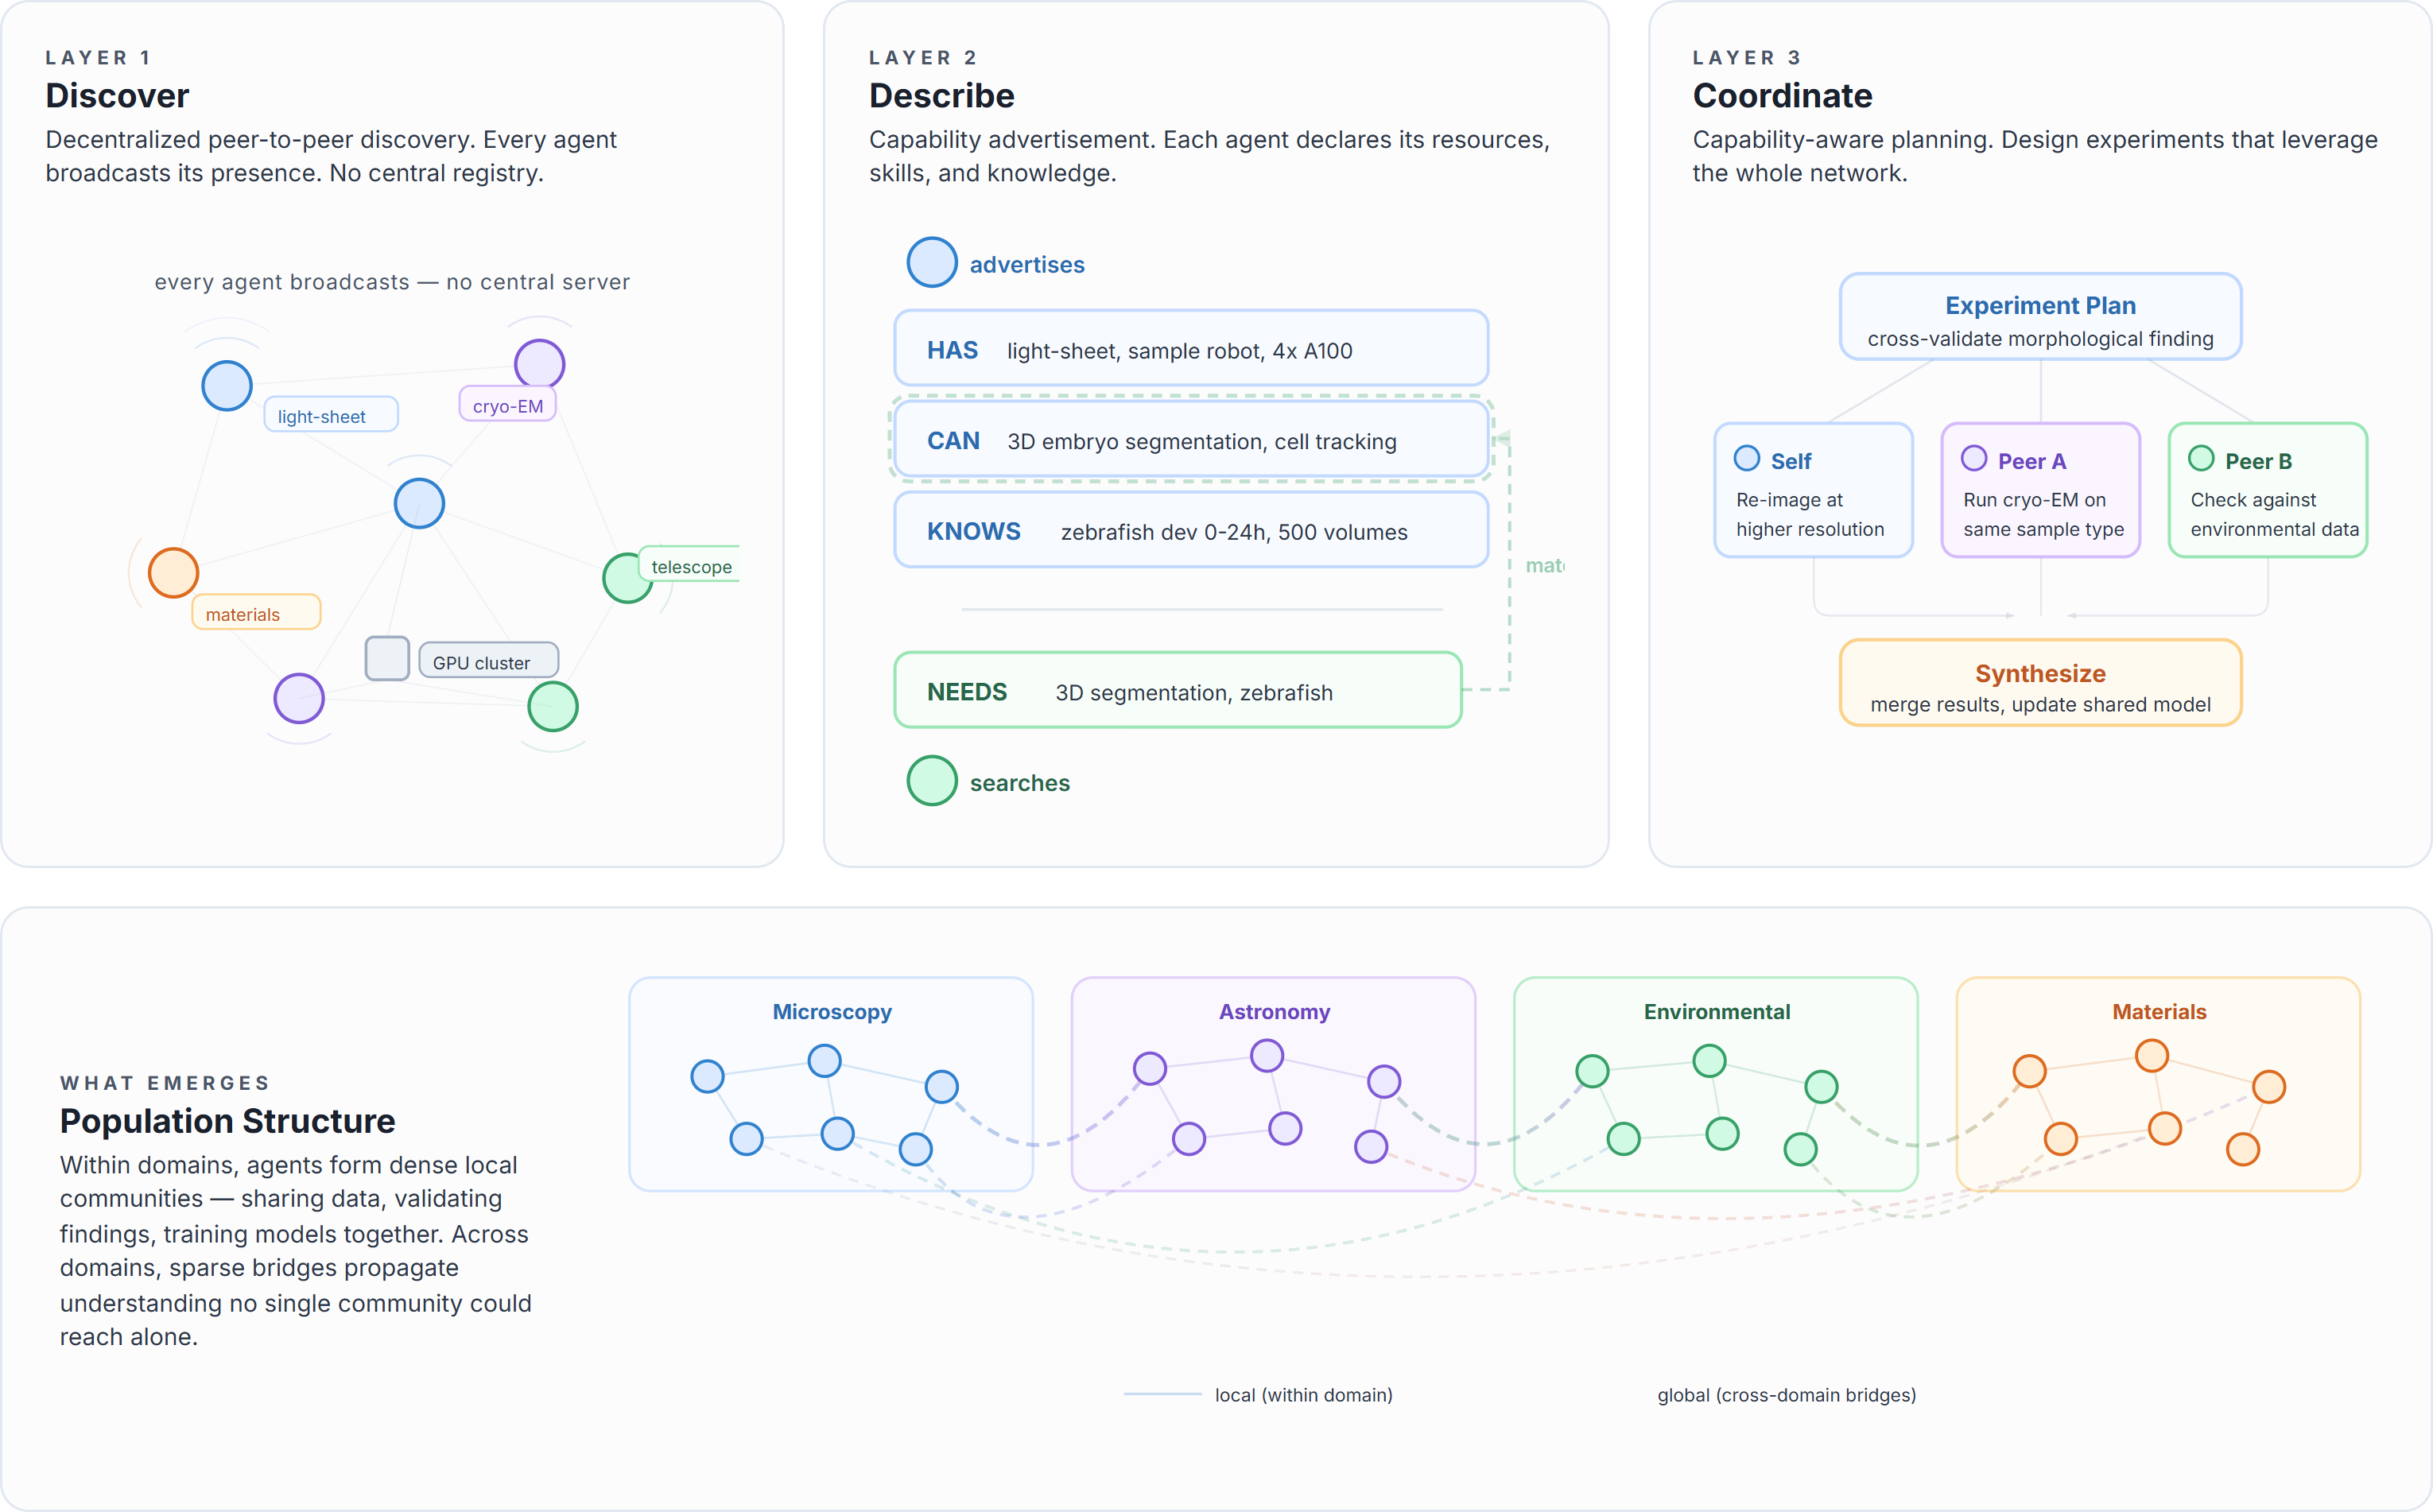
\includegraphics[width=\textwidth]{diagrams/figure2_infrastructure.png}
  \caption{\textbf{Infrastructure and Emergence.}
  \emph{Top}: three infrastructure layers---decentralized discovery, capability advertisement and matching, and coordinated experiment planning.
  \emph{Bottom}: the population structure that emerges---dense local collaboration within domains, sparse cross-domain bridges.}
  \label{fig:infrastructure}
\end{figure}

\section{The Interdisciplinary Promise}

If the epistemic patterns of nature are universal, then the regularities discoverable within one scientific domain should have echoes in others.
Biology and materials science share principles of self-organization.
Astronomy and environmental monitoring share the statistics of rare events in noisy time-series.
These connections exist, but they are difficult for human researchers to make---separated as they are by disciplinary language, publication venues, and institutional structure.

Agentic systems communicating across domains have no such barriers.
An agent trained on microscopy data and an agent trained on astronomical surveys share a common computational substrate.
If the infrastructure supports it, they can exchange not just data but representations, hypotheses, and reasoning patterns.
The result is a natural mixing of scientific cultures---not the forced interdisciplinarity of committee-designed programs, but the organic cross-pollination that emerges when communication barriers fall.

This is why it matters to build the infrastructure with the full vision in mind.
The agentic patterns---perceive, reason, act, record, connect---are domain-agnostic.
The infrastructure layers---discover, describe, coordinate---are general.
What changes across domains is context, not architecture.
Designing for a single instrument or a single domain is straightforward and can be done anywhere.
Designing for the cross-domain case, where agents must negotiate different epistemic traditions and discover universal patterns, is the harder and more consequential problem.

\section{Democratization}

For agentic science to deliver on its promise, the complexity must be invisible to the researcher.
A biologist should not need to understand peer-to-peer protocols to benefit from cross-instrument coordination; a materials scientist should not need to write agent harnesses to share trained models.
The system must meet scientists where they are.

This requires three layers of user-facing design.
First, \textbf{accessible interfaces}: annotation tools that let researchers label data in their native visual language, dashboards that surface agent reasoning in interpretable terms, and APIs that expose capability without exposing machinery.
Second, \textbf{flexible harnesses}: the scaffolding around agents must adapt to different scientific workflows---a microscopy campaign has different rhythms than a materials screening pipeline---while retaining the universal architectural patterns that make cross-domain communication possible.
Third, \textbf{network participation by default}: when a researcher uses the system, their agent joins the network, contributing data, models, and hypotheses to the collective while drawing on the accumulated knowledge of peers.
The value of the system grows with every participant, but the cost of participation must be near zero.

The architecture must therefore be simultaneously domain-flexible and domain-agnostic: flexible enough that each scientific community can shape its tools to local practice, yet universal enough that the infrastructure layer beneath remains a shared substrate for discovery.
This is the crucial lever---not the intelligence of any single agent, but the network effects that emerge when many agents, across many domains, share what they learn.

\section{Implementation}

This program is structured as a 36-month postdoctoral research plan in three phases, building outward from an operational prototype.

\textbf{Phase 1: Two domains, shared infrastructure (months 1--12).}
\textsc{Gently} already operates on a single light-sheet microscope.
Year one deploys it on a second microscopy system and integrates with a genomics pipeline---a natural partner, as genomics is already one of the most agentic fields in biology.
In parallel, we build the inter-agent infrastructure: the discovery and capability advertisement layers, and the data exchange protocols that allow agents to share observations, annotations, and trained models across systems.
On the science side, we develop structured research planning and hypothesis generation for the microscopy--genomics pair, enabling agents to reason across the phenotypic and molecular levels of the same biological system.
Critically, this phase includes a design study for human-in-the-loop governance: annotation tools, validation dashboards, and feedback mechanisms that make it easy for the researcher to assess agent performance, correct its reasoning, and maintain scientific authority over the process.

\textbf{Phase 2: Cross-domain bridges (months 12--24).}
With the biological stack connected, we extend to a non-biological domain.
Materials science is a strong candidate: the field is adopting agentic methods rapidly, and shares with microscopy the core pattern of adaptive observation under physical constraints.
We deploy the infrastructure developed in Phase~1 to connect a materials characterization agent to the existing network, testing whether the discover--describe--coordinate architecture generalizes beyond biology.
Materials characterization also stress-tests two core capabilities: the perception agent, which must adapt its visual reasoning from biological specimens to material microstructures, and the ML pipeline infrastructure, which must support training new models on the fly as the agent encounters unfamiliar imaging modalities and feature spaces.
This phase also matures the democratization tools: refining the APIs and harnesses based on researcher feedback from Phase~1, and lowering the barrier for new instrument types to join the network.

\textbf{Phase 3: Network effects and discovery (months 24--36).}
With agents operating across biology and materials science, we test the central hypothesis: that cross-domain agent coordination surfaces regularities invisible to either community alone.
We focus on federated learning across domains, shared model improvement, and the identification of at least one cross-domain structural or procedural regularity.
The infrastructure and tooling are released as open-source for the broader scientific community.

\end{document}
